\documentclass[../../thesis.tex]{subfiles}

\graphicspath{{Figures/}}

\begin{document}
\chapter{QUBIC Forecasts} \label{chap:forecast}

\ifSubfilesClassLoaded{
    \tableofcontents
}{
    \minitoc
}

\section*{Introduction}

A large part of this thesis has been devoted to the development of realistic simulation and reconstruction pipelines for the QUBIC instrument. In this chapter, we use these pipelines to produce sensitivity forecasts for QUBIC and compare the performance of different reconstruction algorithms, instrumental configurations, and sky models. Although the framework can be extended to more realistic and complex sky models, we deliberately restrict the analysis to relatively simple cases. The primary objective of this thesis was the development and validation of the forecasting pipeline itself, rather than an exhaustive study of the resulting forecasts.

It is important to emphasise that the results presented in this chapter should not be interpreted as predictions of the final performance of the real instrument. Instead, they represent the expected sensitivity of the current simulation and reconstruction framework, based on the present understanding of the instrument. As discussed throughout this thesis, a number of simplifying assumptions have been made, and QUBIC itself is still at the prototype stage. Many aspects of bolometric interferometry remain to be fully understood and validated experimentally, and future developments may significantly modify both the instrumental model and the associated performance forecasts.

\personal{During my first year, I developed with Mathias Regnier the first version of the forecast pipeline, presented within his thesis. During my second and third years, I further developed both FMM and CMM pipelines by improving the overall programming architecture, coding quality, bug corrections and user ergonomics (Chapter~\ref{chap:qubicsoft}) and by studying the TOD realism (Chapter~\ref{chap:tod}).}

\rmk{For now, I consider that I will not have time to add Synchrotron case. I will add them in last minute if I can, otherwise it will only be for the thesis defence.}

\section{Studied Cases}

Different configurations are investigated to assess their impact on the sensitivity of QUBIC, and in particular on the uncertainty of the tensor-to-scalar ratio measurement, $\sigma_r$. We compare different sky models, instrumental configurations, and reconstruction algorithms, and also study the impact of incorporating external data as well as testing the free angular resolution cases.

\subsection{Sky configurations}

Since QUBIC observes the CMB through its $150$ and $220$ GHz channels, we consider sky models containing only the CMB and Galactic dust emission. The contribution from synchrotron emission is neglected, as it mainly contaminates observations at lower frequencies (typically below $100$ GHz)\cite{Krachmalnicoff_2016}. Moreover, we showed in \cite{CMM} that including synchrotron emission in the simulated observations, while not attempting to reconstruct it with the CMM algorithm, introduces only a very small bias on the recovered tensor-to-scalar ratio. This bias remains well below the statistical uncertainty, $\sigma_r$, as illustrated in Figure~\ref{fig:Synchrotron_bias}.

\begin{figure}[!htbp]
    \centering
    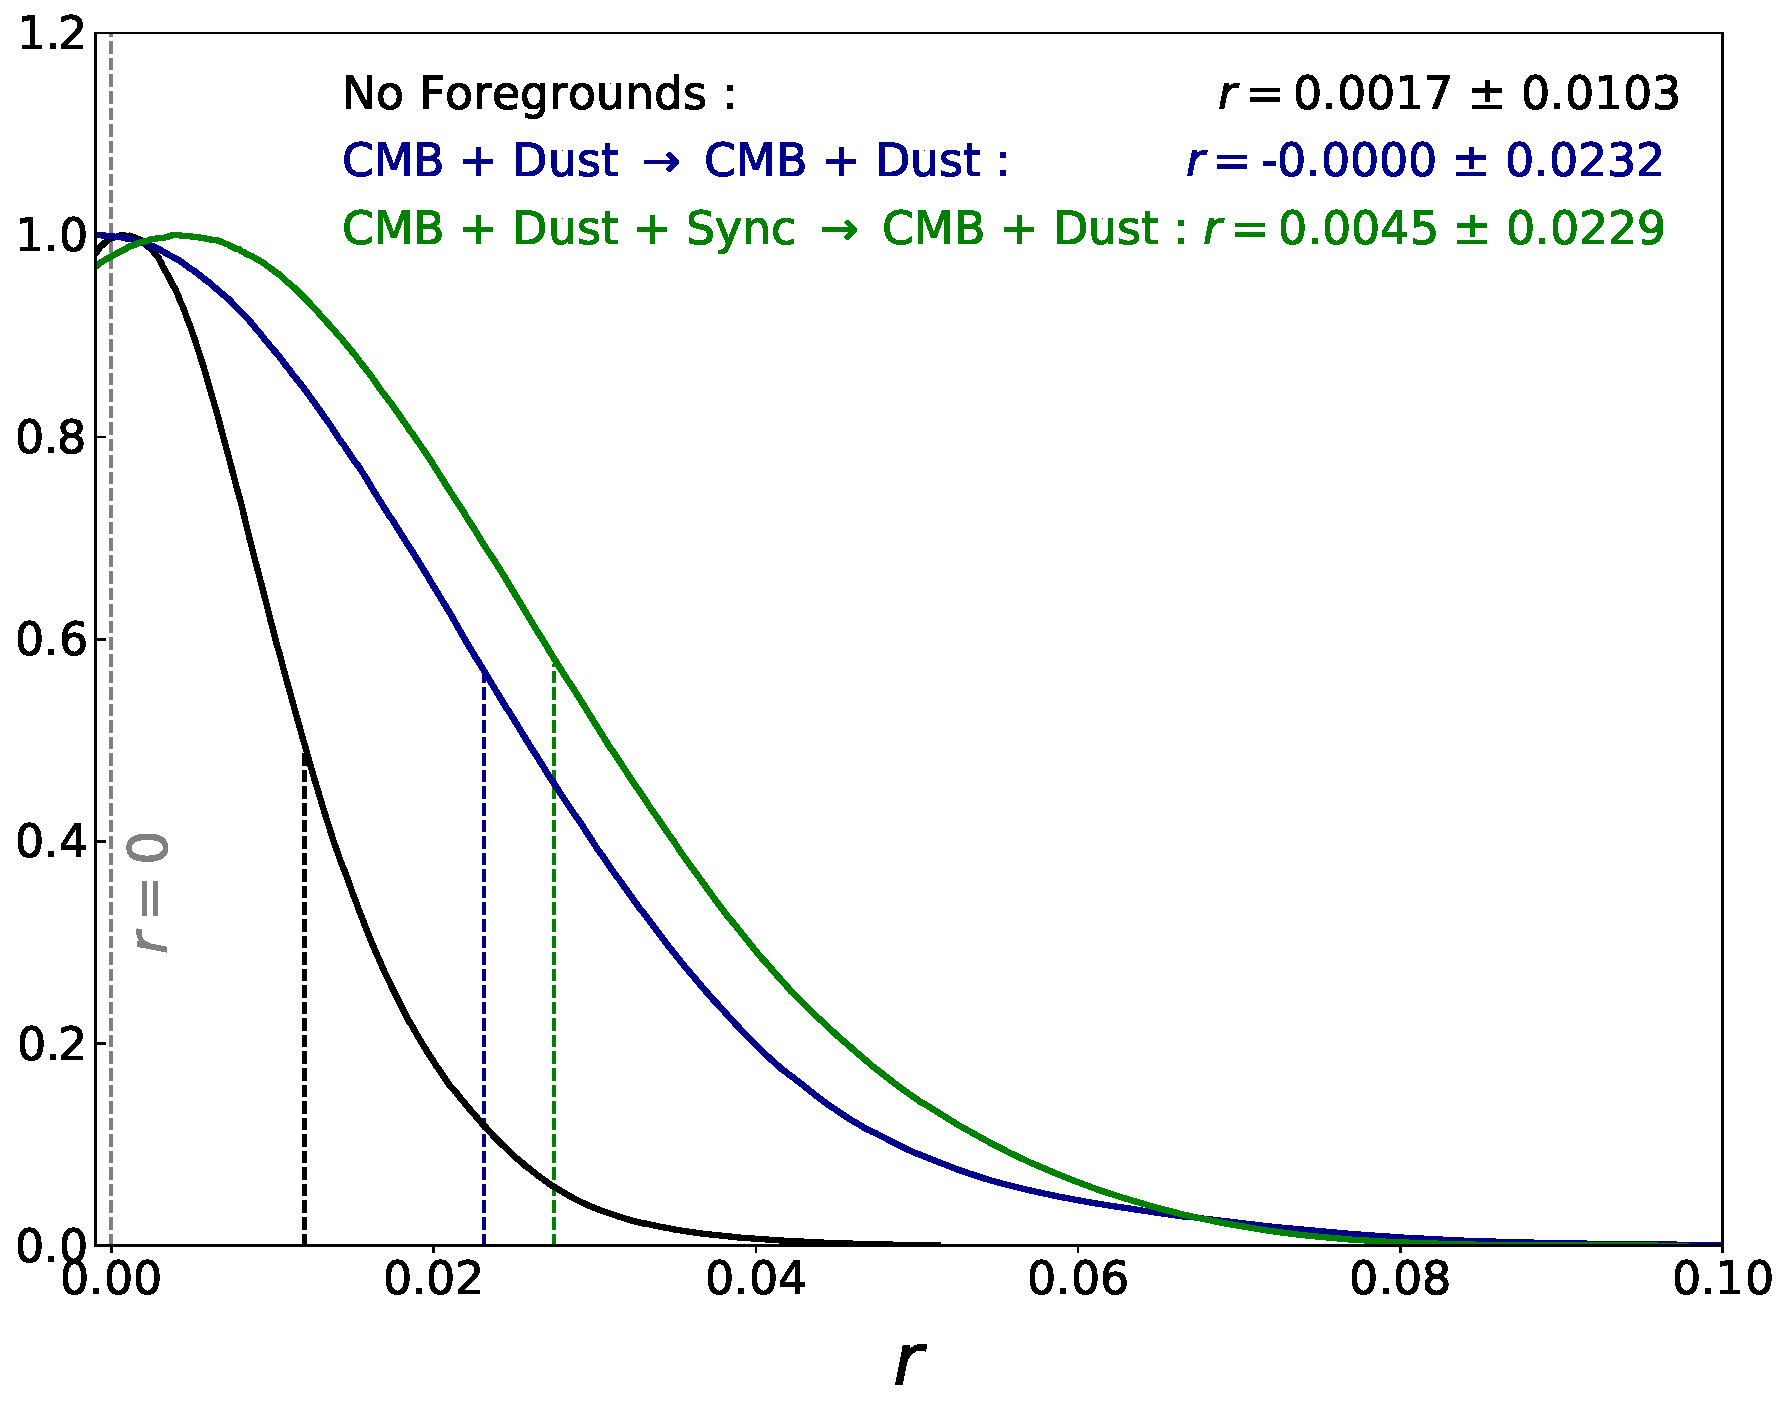
\includegraphics[width=1\linewidth]{sigma_r_triangle.pdf}
    \caption{Posterior distribution of the tensor-to-scalar ratio $r$ obtained with the CMM algorithm for three sky configurations: CMB only, CMB with dust ($d_0$ model), and CMB with dust ($d_0$ model) and synchrotron ($s_0$ model). In the last case, only the CMB and dust components are reconstructed. Neglecting synchrotron during the reconstruction introduces only a small bias on the recovered value of $r$, while the uncertainty $\sigma_r$ remains essentially unchanged. \rmk{Should I keep this figure? The $\sigma_r$ values differ from those presented elsewhere, and I probably won't have time to regenerate it.}}
    \label{fig:Synchrotron_bias}
\end{figure}

Finally, although the more complex dust models $d_1$ and $d_6$ were introduced in Chapter~\ref{chap:CMM}, they are not considered in the forecasts presented in this chapter.

\subsection{Instrumental configurations}

Two instrumental configurations are considered: the Dual Band (DB) and the Ultra Wide Band (UWB) designs, introduced in Chapter~\ref{chap:BI}. Although the DB configuration is no longer considered for the Final Instrument (FI), mainly because of the fabrication and integration challenges associated with the dichroic filter, we include it in the present analysis for two reasons. First, it was the baseline configuration during my Master's internship, and its study motivated the adoption of the UWB as an alternative. Second, it provides a useful reference against which the performance of the UWB design can be assessed. Unlike the DB configuration, the UWB concept fully exploits the specific capabilities of bolometric interferometry, in particular its spectral imaging properties.

Other instrumental configurations are implemented in the simulation framework but are not considered in the present study. These include the Technical Demonstrator (TD), corresponding to the current instrument installed at the observation site, and the Mono Band (MB) configuration. The MB concept was investigated as an alternative after the difficulties encountered with the DB design. In this scenario, the instrument observes at $150$ GHz during part of the total observing time using a single focal plane, before switching to $220$ GHz for the remainder of the observation. The optimal time allocation between the two frequency bands, obtained by minimising $\sigma_r$, was studied by Mathias Regnier during his PhD thesis\cite{mathiasthesis}. Since this configuration is no longer under consideration, it is not discussed further in this thesis.

\subsection{Reconstruction algorithms}

The development of reconstruction algorithms has been one of the main objectives of this thesis. In this section, we compare their performance in terms of the sensitivity to the tensor-to-scalar ratio $r$, quantified by the uncertainty $\sigma_r$.

We first consider the Frequency Map-Making (FMM) algorithm, which reconstructs frequency maps from which the value of $r$ is estimated using the cross-spectrum method described in Chapter~\ref{chap:xspectrum}. FMM can reconstruct multiple frequency maps within the physical bandwidth of QUBIC, controlled by the parameter $N_\text{rec}$. Increasing the number of reconstructed maps is expected to improve the component-separation capabilities by providing additional spectral information. However, it also increases the residual level. The trade-off between these two effects is investigated in this chapter.

We then compare FMM with the Component Map-Making (CMM) algorithm, which jointly performs map-making and component separation by directly reconstructing the astrophysical component maps. As presented in Chapter~\ref{chap:CMM}, two versions of CMM have been developed: the Parametric and Blind approaches. The Parametric approach assumes a physical model for the foreground emission and estimates the associated parameters to build the mixing matrix. In contrast, the Blind approach makes no prior assumption about the foreground model and directly reconstructs the elements of the mixing matrix. We compare the performance of these two approaches with that of FMM, and also investigate the influence of the number of frequencies used to model the mixing matrix, $N_\text{freq}$.

Finally, although the Neural Network Map-Making (NNMM) framework introduced in Chapter~\ref{chap:NNMM} constitutes a promising alternative, no forecast pipeline have been yet developed. It is therefore not included in the comparisons presented in this chapter.

\subsection{External data}

In the FMM framework, we introduced the use of external data to improve the reconstruction at the edges of the observed patch (subsection~\ref{sub:fmm_external_data}). These external information are incorporated only outside the QUBIC field of view so that they do not directly contribute to the estimation of the tensor-to-scalar ratio. Nevertheless, it is advantageous to include external frequency maps, such as those from Planck, in the cross-spectrum analysis. Doing so increases the number of available cross-spectra and strengthens the constraints on the cosmological and foregrounds parameters.

Similarly, the CMM algorithm can benefit from external observations by incorporating additional frequency channels into the mixing matrix, as described in subsection~\ref{sub:cmm_external_data}. In this chapter, we evaluate the impact of including such external data on the sensitivity of the reconstruction.

\rmk{I might not have time to explore this deeply with CMM, as it requires to run the entire CMM to test different addition of Planck bands, while it is just a different fit for the FMM, so few minutes to compute $\sigma_r$.}

\subsection{Free angular resolution}

In Chapters~\ref{chap:FMM} and~\ref{chap:CMM}, we introduced a reconstruction strategy in which the angular resolution is allowed to vary freely during the map-making process (subsections~\ref{sub:fmm_convolution} and~\ref{sub:cmm_free_convo}). This approach significantly reduces the computational cost by avoiding repeated beam convolutions during the iterative reconstruction. However, before adopting it for forecasting studies, it is important to verify that this approximation does not degrade the final sensitivity of the instrument. In this chapter, we therefore compare the performance obtained with fixed and free angular resolution assumptions.

\section{Results}

\subsection{Compare QUBIC configurations} \label{sub:design_comparison}

\subsection{Dual bands without spectral imaging: \enquote{Imager case}}

\subsection{Dual bands with spectral imaging: \enquote{BI case}}

\subsection{Ultra-wide band: \enquote{Extreme BI case}}

\subsection{Successive mono-band case: \enquote{Conservative case}}

\section{Compare QUBIC's map-making algorithms}

\subsection{FMM: Cross-spectra Analysis}

\subsection{NN-FMM: Cross-spectra Analysis}

\subsection{CMM: Parametric Analysis}

\subsection{NN-CMM: Parametric Analysis}

\subsection{CMM: Blind Analysis}

\subsection{Addition of external data for component separation}

\end{document}